\begin{frame}{Biological Analogy}
    \begin{figure}[H]
		\centering
		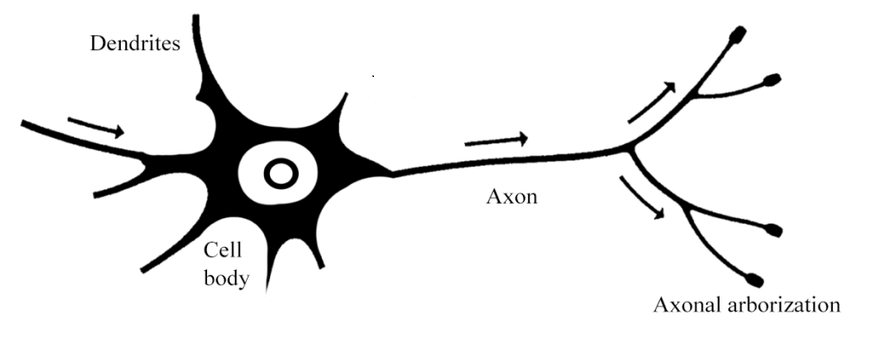
\includegraphics[width=0.9\textwidth]{Figs/biological_neuron.png}
		\caption{Anatomy of a biological neuron \cite{biological-and-nn-neuron}.}
	\end{figure}
\end{frame}

\begin{frame}{Biological analogy}
    \begin{figure}[H]
		\centering
		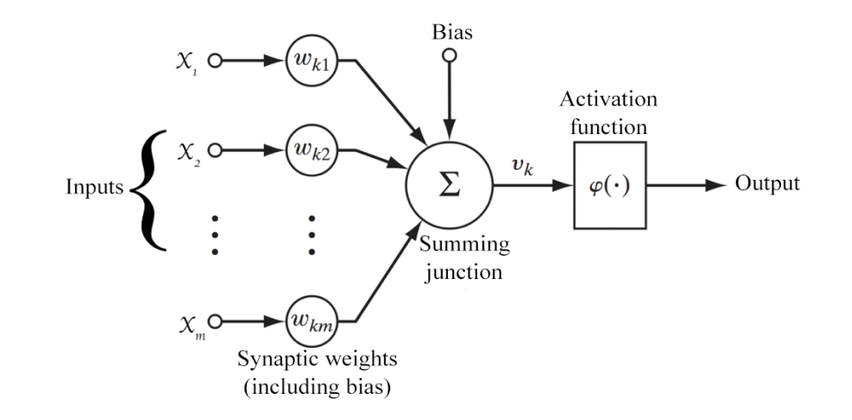
\includegraphics[width=0.9\textwidth]{Figs/nn_neuron.png}
		\caption{Neural network neuron \cite{biological-and-nn-neuron}.}
	\end{figure}
\end{frame}

\begin{frame}{Activation Functions}
    \begin{figure}[H]
		\centering
		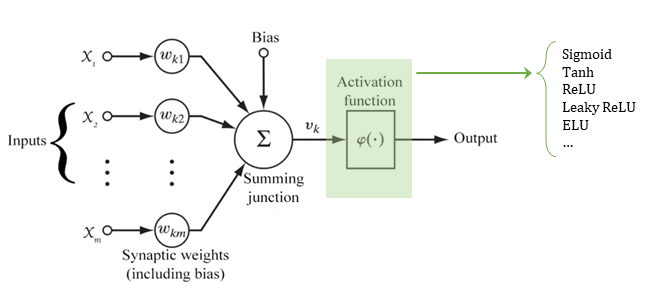
\includegraphics[width=0.9\textwidth]{Figs/activation_function_1.png}
		\caption{Activation function}
	\end{figure}
\end{frame}

\begin{frame}{Activation Functions}
    \begin{figure}[H]
		\centering
		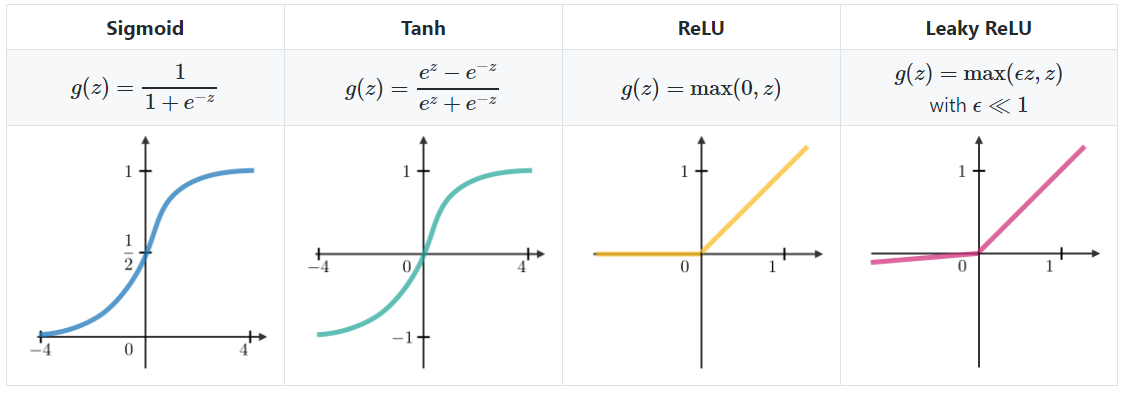
\includegraphics[width=0.9\textwidth]{Figs/activation_function_2.png}
		\caption{Activation functions \cite{activation-functions}.}
	\end{figure}
\end{frame}

\begin{frame}{Gradient Descent}
    \begin{figure}[H]
		\centering
		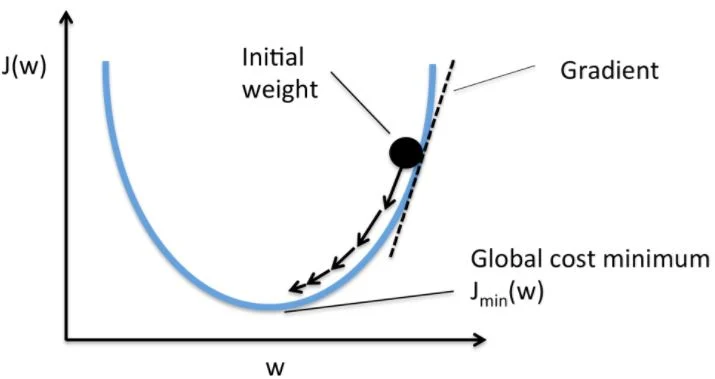
\includegraphics[width=0.70\textwidth]{Figs/gradient_descent2.png}
		\caption{Gradient descent \cite{gradient-descend2}.}
	\end{figure}
\end{frame}

\begin{frame}{Gradient Descent}
% 	Assuming cost function $J(w)$ as the sum of squared errors (SSE)
	\begin{center}
	    $J(\mathbf{w})  = \frac{1}{2} \sum_{i} (\text{target}^{(i)} - \text{output}^{(i)})^2 \quad \quad \text{output}^{(i)} \in \mathbb{R}$
	    
	    \vspace{5}
	    
	    \begin{equation*} 
            \begin{split}
                \frac{\partial J}{\partial w_j} & = \frac{\partial }{\partial w_j} \frac{1}{2} \sum_i  (t^{(i)} - o^{(i)})^2 \\
                 & = \frac{1}{2} \sum_i \frac{\partial}{\partial w_j} (t^{(i)} - o^{(i)})^2 \\
                 & = \frac{1}{2} \sum_i 2 (t^{(i)} - o^{(i)}) \frac{\partial}{\partial w_j} (t^{(i)} - o^{(i)}) \\ 
                 & = \sum_i (t^{(i)} - o^{(i)}) \frac{\partial}{\partial w_j} \bigg(t^{(i)} - \sum_j w_j x^{(i)}_{j}\bigg) \\
                 & = \sum_i  (t^{(i)} - o^{(i)})(-x^{(i)}_{j}) 
             \end{split}
        \end{equation*}
        
        
        \vspace{5}
        
        $\Delta w_j = - \eta \frac{\partial J}{\partial w_j} = - \eta \sum_i  (t^{(i)} - o^{(i)})(- x^{(i)}_{j}) = \eta \sum_i (t^{(i)} - o^{(i)})x^{(i)}_{j}$
        
        
        $\mathbf{w} := \mathbf{w} + \Delta \mathbf{w}$

	\end{center}
	
\end{frame}
